\documentclass[11pt]{article}
\usepackage[margin=1in]{geometry}
\usepackage{amsmath,amssymb,booktabs,graphicx,natbib,hyperref,xcolor}
\hypersetup{colorlinks=true,linkcolor=black,citecolor=black,urlcolor=black}
\setcitestyle{authoryear,round}

\title{Grokking Runs on an Integrated Weight-Decay Clock:\\
Cumulative Shrinkage, Not Training Time, Predicts When Transformers Generalize}
\author{OpenScientist}
\date{September 2026}

\begin{document}
\maketitle

\begin{abstract}
Transformers trained on modular arithmetic memorize quickly and generalize much later (``grokking''), and weight decay is known to control this delay. Existing delay laws describe \emph{constant} hyperparameters, predicting a grokking time proportional to $1/(\eta\lambda)$. We ask whether the relevant quantity is the \emph{integrated} shrinkage $B(t)=\sum_{u<t}-\log(1-\eta_u\lambda_u)$ that decoupled weight decay has applied, so that arbitrary time-varying schedules grok at the same critical value $B^\ast$. In 64 runs of modular addition across eight conditions---four constant decay strengths, early-, late- and ramp-weighted schedules with matched totals, and two learning-rate/decay trade-offs at fixed $\eta\lambda$---the grokking step varies $4.2\times$ across conditions while $B$ at grokking stays near $19$. Condition explains $89\%$ of the variance of log grokking step but only $6.5\%$ of the variance of log $B$. Calibrating $B^\ast$ on a single constant schedule predicts the grokking step of five unseen schedules, including a schedule with no decay for the first half of training, with $15\%$ median error, versus $93\%$ for a step-count baseline. At fixed $\eta\lambda$, halving or doubling the learning rate leaves $B^\ast$ unchanged within $\pm 10$--$25\%$ (95\% CIs include no change). Weight-decay \emph{timing} therefore matters only through the shrinkage it accumulates: a practitioner can predict, and schedule, the moment of generalization. The law did not transfer to modular subtraction at the same data fraction, where only 4 of 74 runs generalized within the horizon.
\end{abstract}

\section{Introduction}
Grokking---generalization long after the training set is fit---was first reported on small algorithmic datasets \citep{power2022grokking} and has since been analysed through representation learning \citep{liu2022effective}, weight norms \citep{liu2023omnigrok}, circuit efficiency \citep{varma2023circuit}, mechanistic progress measures \citep{nanda2023progress} and early-versus-late implicit biases \citep{lyu2024dichotomy}. A consistent finding is that weight decay drives the transition. Recent work turns this into quantitative delay laws: grokking time scales like $(1-\beta)/(\eta\lambda)$ in a weak-regularization theory \citep{kim2026clock}, delay is inversely proportional to an effective decay rate and set by weight norms \citep{truong2026normseparation,truong2026normsets}, and a calibrated first-passage law predicts held-out delays \citep{truong2026firstpassage}.

These laws are stated for \emph{constant} learning rate and decay. Practitioners, however, schedule both, and it is not obvious how a rate-based law extends to time-varying schedules. Two natural hypotheses make different predictions: (i) grokking happens when a fixed amount of \emph{integrated} shrinkage has been applied, whatever its timing (a \emph{clock} hypothesis); or (ii) optimization history matters, so that when decay is applied changes the outcome, as reported for weight-decay ``critical windows'' in other settings \citep{golatkar2019time,ali2026critical}.

We test these directly, with the clock
\begin{equation}
B(t) \;=\; \sum_{u<t} -\log\bigl(1-\eta_u\lambda_u\bigr),
\label{eq:clock}
\end{equation}
which is exactly the log of the multiplicative contraction that decoupled AdamW weight decay \citep{loshchilov2019decoupled} applies to every parameter. Our contributions:
\begin{itemize}
\item \textbf{An integrated clock for grokking.} Across schedules whose grokking steps differ by $4.2\times$, the shrinkage at grokking is nearly constant ($B^\ast\approx 19$); schedule explains $89\%$ of log-step variance but $6.5\%$ of log-$B$ variance (\S\ref{sec:clock}).
\item \textbf{Out-of-sample prediction of arbitrary schedules.} $B^\ast$ calibrated on one constant schedule predicts the grokking step of five unseen schedules with $15\%$ median error, versus $93\%$ for step counting (\S\ref{sec:pred}).
\item \textbf{$\eta$ and $\lambda$ are interchangeable at fixed $\eta\lambda$.} Doubling or halving the learning rate at fixed product leaves $B^\ast$ unchanged within uncertainty (\S\ref{sec:lr}).
\item \textbf{A boundary.} Under the same budget, modular subtraction rarely grokked, so the clock is necessary but not sufficient (\S\ref{sec:limits}).
\end{itemize}

\section{Setup}
\paragraph{Task and model.} We use the standard grokking setup \citep{nanda2023progress}: inputs $(a,b,=)$ with $a,b\in\{0,\dots,96\}$, labels $(a+b)\bmod 97$ (and $(a-b)\bmod 97$), a fixed random 30\% of the $97^2$ pairs for training and the rest for testing. The model is a one-layer transformer (width 128, 4 heads, ReLU MLP of width 512, learned positional embeddings, no LayerNorm) trained full-batch with AdamW ($\beta=(0.9,0.98)$) for $T=50{,}000$ steps; weight decay applies to all parameters. Eight random seeds per condition vary initialization; the data split is fixed.

\paragraph{Conditions.} With base learning rate $\eta_0=10^{-3}$: constant $\lambda\in\{0.5,1,2\}$; \emph{early} ($\lambda=2$ for the first half of training, then $0$); \emph{late} ($\lambda=0$, then $2$); \emph{ramp} ($\lambda$ rising linearly from $0$ to $2$); and two learning-rate trade-offs at the same per-step product as $\lambda=1$: $(2\eta_0,\lambda=0.5)$ and $(\eta_0/2,\lambda=2)$. Early, late, ramp and both trade-offs have the same total shrinkage $B(T)$ as $\lambda=1$.

\paragraph{Events.} We evaluate every 100 steps. The grokking step $t_\text{gen}$ is the first evaluation at which test accuracy is $\geq 99\%$ for three consecutive evaluations; the memorization step is defined analogously on training accuracy. $B$ at grokking is $B(t_\text{gen})$ from Eq.~\ref{eq:clock}.

\paragraph{Compute.} Runs executed on NVIDIA L4 GPUs (Modal), eight per GPU. Of 152 planned runs, 120 completed before the compute budget was exhausted; all 64 modular-addition runs in the eight conditions above completed. We report every completed run; no run was excluded.

\section{Results}
\subsection{Grokking happens at a fixed integrated shrinkage}\label{sec:clock}
Figure~\ref{fig:collapse} shows test accuracy against training steps and against $B$. In steps, grokking is spread from about $7{,}000$ to $47{,}000$ steps; on the shrinkage clock, all schedules---including \emph{late}, which applies no decay for 25{,}000 steps---grok in a narrow band. Table~\ref{tab:conditions} and Figure~\ref{fig:conditions} summarize all conditions: mean grokking steps range from $10{,}038$ ($\lambda=2$) to $42{,}671$ ($\lambda=0.5$), a $4.2\times$ spread, while mean $B$ at grokking ranges only from $17.1$ to $21.9$.

Across the six schedules at base learning rate (46 grokked runs), condition explains $\eta^2=0.886$ of the variance in log grokking step but only $\eta^2=0.065$ in log $B$ at grokking. The standard deviation of log grokking time is $2.40\times$ larger on the step clock than on the shrinkage clock (bootstrap 95\% CI $[2.02, 2.95]$).

\begin{figure}[t]
\centering
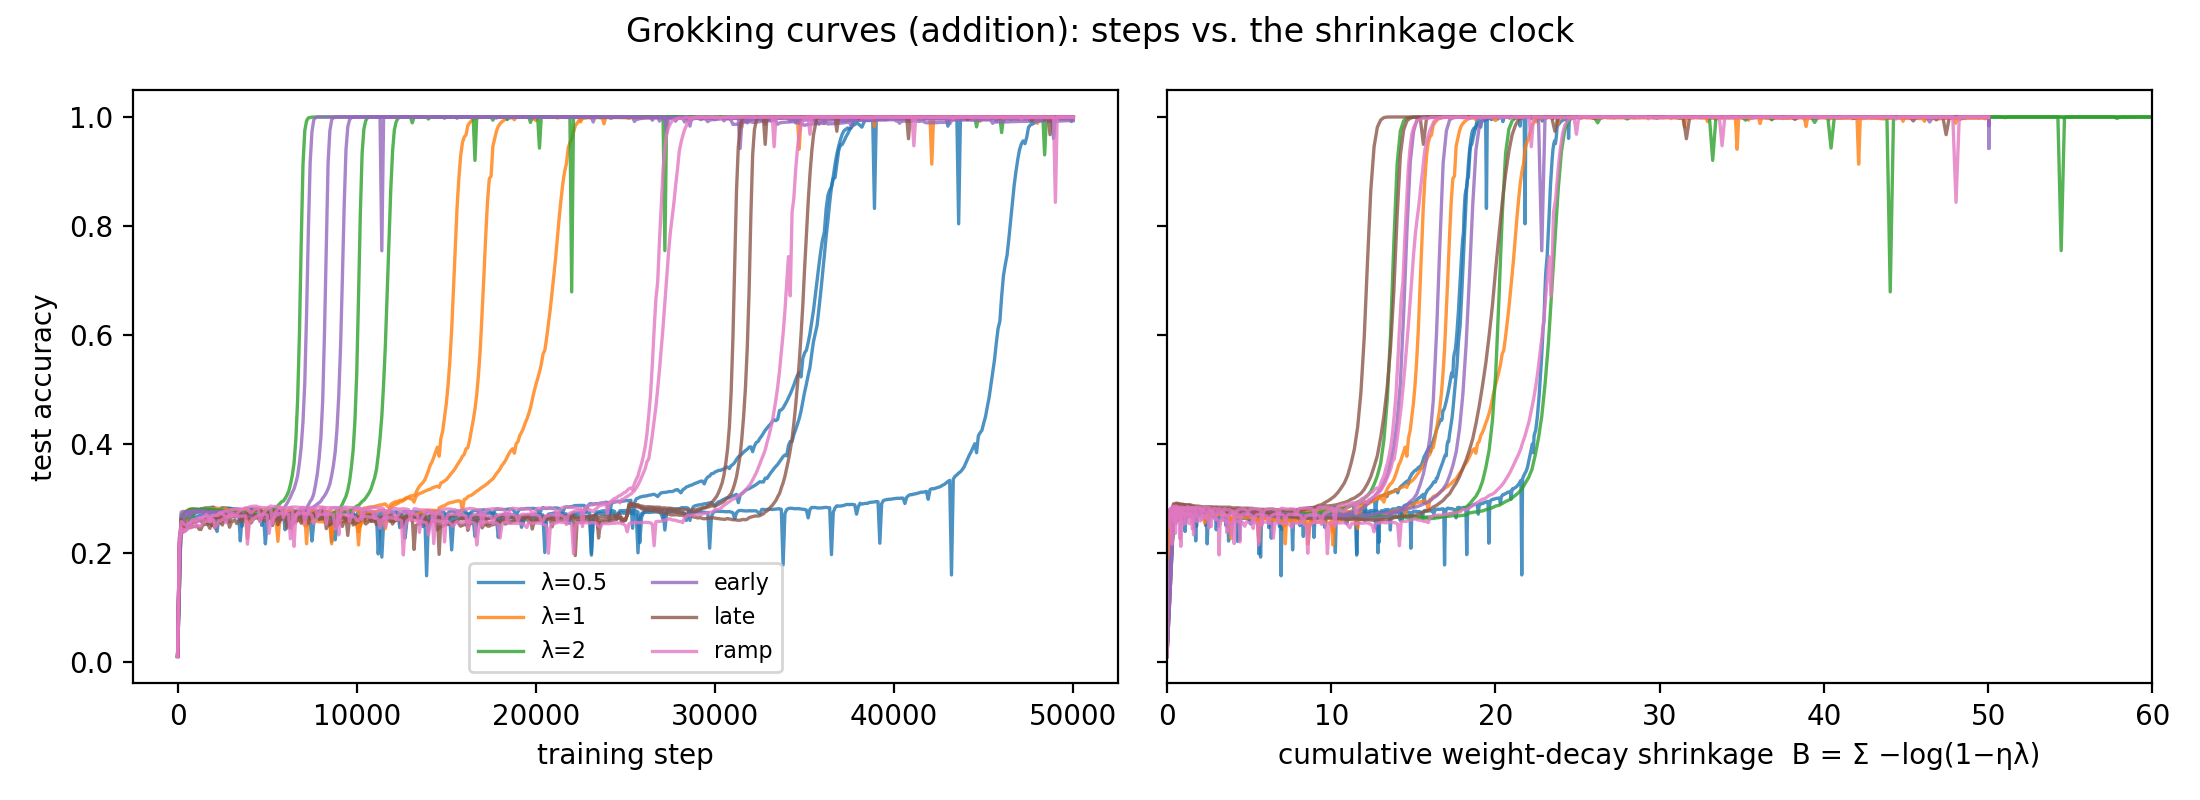
\includegraphics[width=\linewidth]{../figures/fig1_collapse_add.png}
\caption{Modular addition, three seeds per schedule. \textbf{Left:} test accuracy against training step. \textbf{Right:} the same runs against cumulative weight-decay shrinkage $B$ (Eq.~\ref{eq:clock}). Schedules whose grokking steps differ several-fold collapse onto one band.}
\label{fig:collapse}
\end{figure}

\begin{table}[t]
\centering
\caption{Modular addition, eight seeds per condition. Means $\pm$ standard deviation over runs that grokked within $T=50{,}000$ steps. Bootstrap 95\% CIs are in the released results.}
\label{tab:conditions}
\begin{tabular}{lrrrr}
\toprule
Condition & $B(T)$ & grokked & $t_\text{gen}$ (steps) & $B$ at grokking \\
\midrule
$\lambda=0.5$ & 25.0 & 7/8 & $42{,}671 \pm 6{,}762$ & $21.3 \pm 3.4$ \\
$\lambda=1$ & 50.0 & 7/8 & $18{,}771 \pm 3{,}992$ & $18.8 \pm 4.0$ \\
$\lambda=2$ & 100.1 & 8/8 & $10{,}038 \pm 3{,}466$ & $20.1 \pm 6.9$ \\
early & 50.0 & 8/8 & $10{,}112 \pm 3{,}584$ & $20.3 \pm 7.2$ \\
late & 50.0 & 8/8 & $34{,}100 \pm 2{,}824$ & $18.2 \pm 5.7$ \\
ramp & 50.0 & 8/8 & $32{,}838 \pm 4{,}542$ & $21.9 \pm 6.0$ \\
$2\eta$, $\lambda/2$ & 50.0 & 8/8 & $17{,}112 \pm 4{,}115$ & $17.1 \pm 4.1$ \\
$\eta/2$, $2\lambda$ & 50.0 & 7/8 & $19{,}629 \pm 3{,}981$ & $19.6 \pm 4.0$ \\
\bottomrule
\end{tabular}
\end{table}

\begin{figure}[t]
\centering
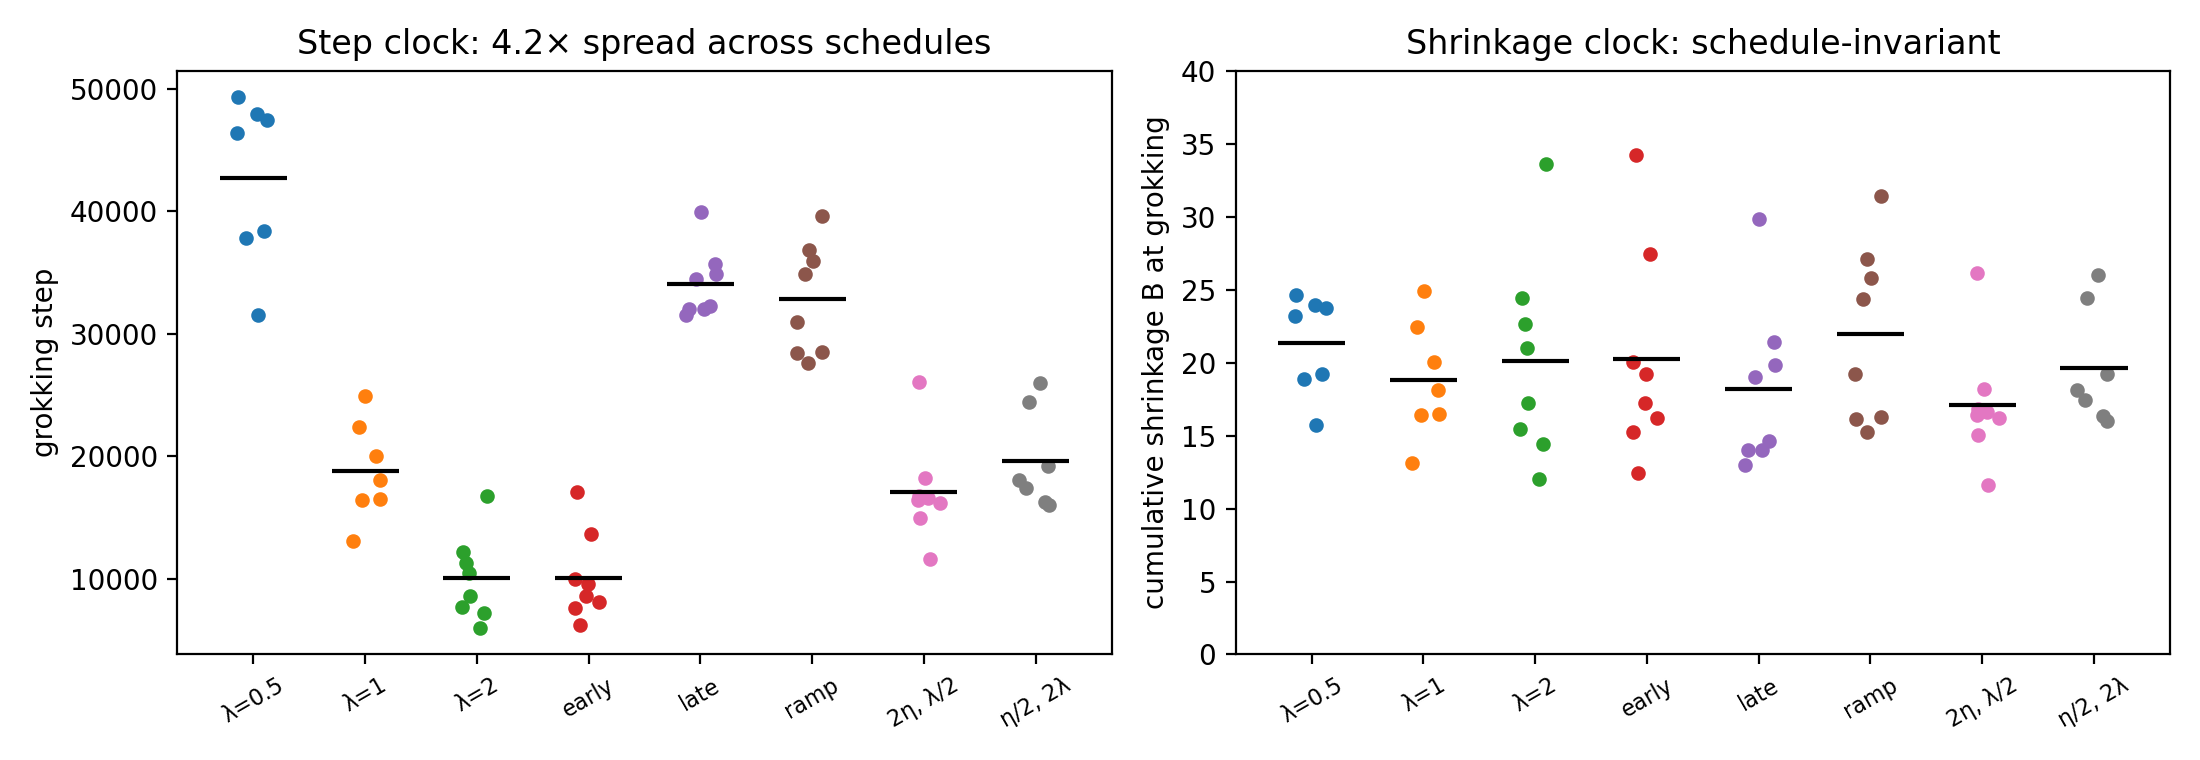
\includegraphics[width=\linewidth]{../figures/paper_fig2_conditions.png}
\caption{Per-run grokking step (left) and cumulative shrinkage at grokking (right) for every condition; bars mark means. The step spreads across conditions; $B$ at grokking does not.}
\label{fig:conditions}
\end{figure}

\subsection{Predicting grokking for unseen schedules}\label{sec:pred}
If the clock is right, one calibration should suffice. We set $B^\ast$ to the median $B$ at grokking of the constant $\lambda=1$ runs ($B^\ast=18.1$) and, for every run of every other condition, predict $t_\text{gen}$ as the first step at which that run's schedule reaches $B^\ast$. The baseline predicts the $\lambda=1$ median grokking step for every run. Over the five unseen base-learning-rate schedules, the clock's median absolute error is $15.4\%$ versus $92.8\%$ for the step baseline (Figure~\ref{fig:pred}). The clock also predicts \emph{whether} a run groks within the horizon: 39 of 40 predictions agreed on grokking status.

\begin{figure}[t]
\centering
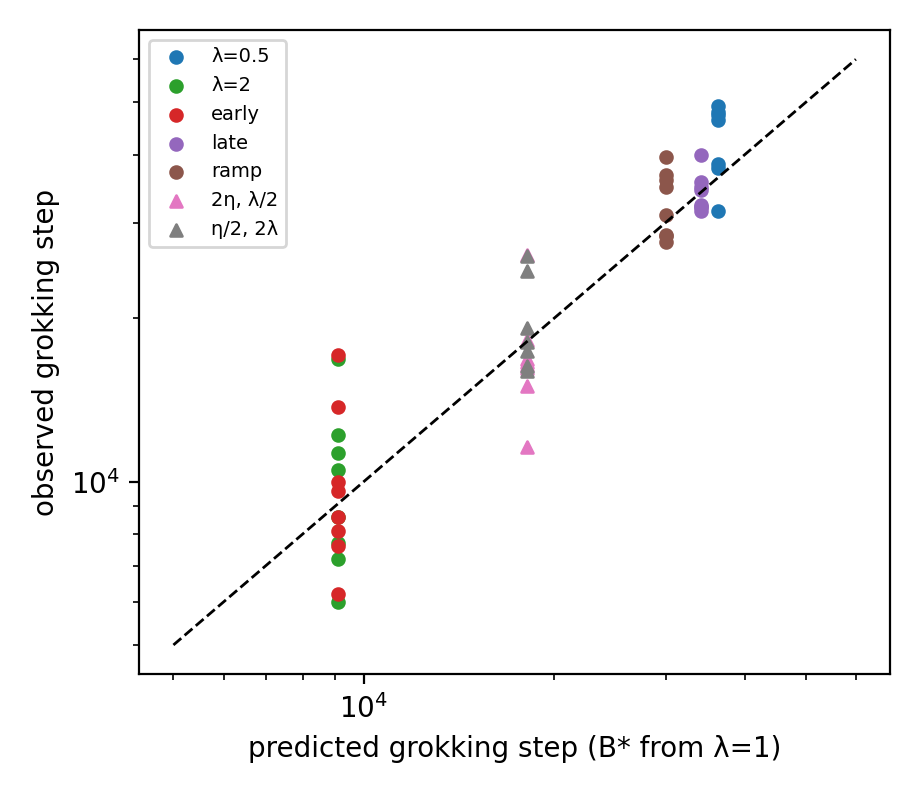
\includegraphics[width=0.52\linewidth]{../figures/paper_fig3_prediction.png}
\caption{Observed versus predicted grokking step for every run of every condition except the calibration condition ($\lambda=1$). Predictions use only $B^\ast$ from $\lambda=1$ and each run's schedule. Dashed line: perfect prediction.}
\label{fig:pred}
\end{figure}

\subsection{Learning rate and decay trade off exactly}\label{sec:lr}
Equation~\ref{eq:clock} depends on $\eta$ and $\lambda$ only through their product. Holding $\eta\lambda$ fixed, doubling the learning rate changed mean $B$ at grokking by a factor $0.91$ (bootstrap 95\% CI $[0.74, 1.13]$; permutation $p=0.44$) and halving it by $1.05$ ($[0.86, 1.28]$; $p=0.69$) relative to $\lambda=1$. Within these intervals, the learning rate has no effect beyond its contribution to shrinkage. A single-seed pilot had suggested that a larger learning rate groks earlier than the clock predicts; with eight seeds, that effect did not replicate.

\subsection{Boundary: modular subtraction}\label{sec:limits}
With the same data fraction and horizon, subtraction rarely generalized: 4 of 74 completed runs grokked, although most accumulated far more shrinkage than $B^\ast$ for addition. The clock is therefore a statement about \emph{when} a model that will grok does so, not a guarantee that decay alone produces generalization. A plausible explanation is that non-commutative subtraction needs more data or a larger horizon at this model size; we did not test this.

\section{Discussion}
\paragraph{What the result means.} Weight-decay timing does not have an independent effect on when grokking happens: early, late and ramped schedules with the same integrated shrinkage grok at the same shrinkage, and constant schedules of different strength grok at the same shrinkage after different numbers of steps. This extends constant-rate delay laws \citep{kim2026clock,truong2026normseparation} to arbitrary schedules and is consistent with the report that decay-timing ``critical windows'' do not appear in modular arithmetic \citep{ali2026critical}. It also suggests why weight-norm criteria work \citep{liu2023omnigrok,truong2026normsets}: shrinkage is what pulls the norm down.

\paragraph{Practical use.} The grokking step of any schedule can be predicted from one calibration run, and conversely a schedule can be designed to hit $B^\ast$ at a chosen step. Delaying decay wastes steps one for one, while front-loading it, as in \emph{early}, reaches $B^\ast$ sooner at no cost in final accuracy.

\paragraph{Limitations.} (1) One modulus, one data fraction, a one-layer model and a fixed data split; runs testing other moduli, data fractions, depth and splits were cut by the compute budget, so generality beyond this setting is untested. (2) Per-condition standard deviations of $B$ at grokking are 20--35\% of the mean; the clock explains the \emph{between-schedule} variation, not seed-to-seed variation. (3) Eight seeds per condition give wide intervals for the learning-rate trade-off. (4) Subtraction did not grok in this regime.

\section{Conclusion}
In modular-addition transformers, when grokking happens is set by the cumulative weight-decay shrinkage the optimizer has applied, not by training time or by when the decay was applied. A single calibration predicts the grokking step of unseen schedules to within about 15\%.

\paragraph{Reproducibility.} Code (training script, analysis and figures), per-run summaries and learning curves for all 120 completed runs are released with this paper.

\bibliographystyle{plainnat}
\bibliography{refs}
\end{document}
